\subsection{Statistique et alignement}

Une autre approche qui peut être combinée à celle des graphes est l'utilisation des statistiques pour comparer les génomes. Avec l'ensemble des séquences disponibles, il est plutôt sensé de penser que lorsqu'on veut comparer une nouvelle séquence à celles disponibles, celle-ci s'alignera sur un sous-ensemble de séquences qui sont déjà connues pour être similaires. L'idée sera donc de créer des groupes de séquences similaires pour ensuite établir une représentation ou un modèle statistique de cet ensemble. Ce modèle représentera alors les fréquences de chaque résidu pour une position donnée, et donc représenter la "séquence" consensus de l'ensemble des séquences regroupées. 

\subsubsection{Partitionnement des séquences par similarité. }

Les méthodes de partitionnement, ou clustering en anglais, reposent sur les méthodes d'alignement pour déterminer la similarité des séquences, et les graphes pour représenter les liens de similarités entre chaque séquence. 

De manière générale, on va regrouper les séquences en groupes d'homologues en utilisant un seuil de similarité plus ou moins élevé. Les outils sont régulièrement présentés en utilisant la séquence protéique plutôt que nucléique pour calculer la similarité. Ce choix permet de réduire la complexité tout en étant plus précis sur l'évaluation de la similarité fonctionnelle et structurelle. Dans ce cas, il faudra faire attention à la nuance entre similarité et identité. Ce qui va varier entre les méthodes, c'est l'algorithme de partitionnement utilisé. Le \autoref{tab:clustering} présente un aperçu des méthodes et des outils existants.  

\begin{longtable}{|p{0.14\textwidth}|p{0.25\textwidth}|p{0.25\textwidth}|p{0.25\textwidth}|}
\hline
\textbf{Outil} & \textbf{Description} & \textbf{Avantages} & \textbf{Inconvénients} \\
\hline
COGs & Classification basée sur l'évolution. Les clusters obtenus sont des clusters de protéines orthologues & Larges base de données, bien documenté et très utilisé & Méthode statique, pas mise à jour régulièrement. \\
\hline
CD-HIT & Partitionnement rapide, ordonnant les protéines de la plus longue à la plus courte & Très rapide, efficace pour la réduction de redondance & Sensibilité limitée sur de faibles identités \\
\hline
InParanoid & Détection de paralogues et d'orthologues. & Fiable pour la détection des orthologues proches. Discerne bien les paralogues des orthologues & Moins adaptés aux comparaisons de nombreux génomes\\
\hline
OrthoMCL & Construit des groupes d'orthologues et identifie-les paralogues récent. & Bonne précision et adaptation à divers organismes & Plus lents sur de gros ensembles de données \\
\hline
UBLAST / USEARCH / UCLUST & Alignement et clustering rapide & Très rapide et peu gourmand en mémoire & Moins précis que BLAST sur certaines comparaisons \\
\hline
FastOrtho & Version rapide d'OrthoMCL & Plus rapide sur de gros ensembles & Peut perdre en précision par rapport à OrthoMCL \\
\hline
Proteinortho & Détection rapide d'orthologues & Évolutif pour de nombreux génomes & Moins de détails sur les relations fonctionnelles \\
\hline
OMA & Approche évolutive d'orthologie & Haute précision sur les génomes bien annotés & Temps de calcul important sur de grands jeux de données \\
\hline
BUSCO & Évaluation de la complétude des génomes & Excellente référence pour les nouveaux génomes & Ne permet pas une recherche d'orthologues à grande échelle \\
\hline
\caption[Outils de clustering des séquences]{Présentation des principaux  outils de clustering de séquences avec leurs descriptions, avantages et inconvénients. Références des outils : \cite{tatusov_genomic_1997,li_sequence_2002}}
\label{tab:clustering}
\end{longtable}

\subsubsection{MMSeqs2}

Un outil que j'ai utilisé à de nombreuses reprises dans mes travaux est l'outil MMSeqs2 \cite{steinegger_mmseqs2_2017}. L'objectif de MMSeqs2 est de partitionner les séquences en groupe d'homologue, de manière rapide et efficace.

Contrairement à d'autres outils (\autoref{tab:clustering}), dans son étape d'alignement, MMSeqs2 ne va pas faire des comparaisons exactes de k-mers, mais il va chercher des k-mers similaires. Cette différence permet de comparer les k-mers plus rapidement tout en utilisant des k-mers de plus grandes tailles, améliorant sa sensibilité\footnote{La sensibilité correspond au nombre de séquences qui sont alignés par rapport au nombre de séquences qui sont similaires.}. Comme présenté sur la \autoref{fig:mmseqs2}, les k-mers utilisés sont "espacés", ce qui permet un recouvrement plus important de la séquence et donc de réduire les alignements liés au hasard de k-mers successif entre 2 séquences non homologues. S'appuyant sur cette caractéristique, les auteurs de MMSeqs2 vont supposer que si les séquences ont des k-mers similaires, séparé par le même nombre de résidus, alors la zone entre les k-mers à des chances de s'aligner, ce qui permet d'étendre les zones alignables (diagonale). Enfin, un score est associé aux diagonales, et va être utilisé pour filtrer les séquences qui ont le plus de probabilités de s'aligner. Pour terminer, MMSeqs2 va également s'appuyer sur les technologies informatiques, aussi bien matériel que logiciel, pour optimiser les ressources utilisé. Les alignements peuvent être distribués à plusieurs c\oe urs\footnote{Le c\oe urs est la partie du processeur qui permet d'exécuter une instruction.}. Aussi, MMseqs2 ne nécessitant pas d'accès aléatoire à la mémoire dans sa boucle interne, sa durée d'exécution est presque inversement proportionnelle au nombre de c\oe urs utilisés.

\begin{figure}[htbp]
    \centering
    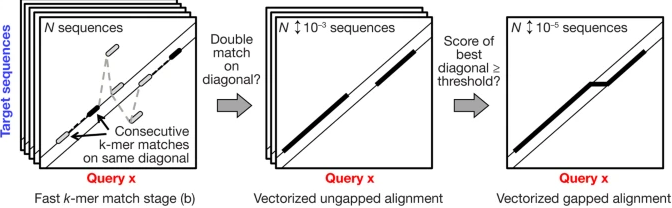
\includegraphics[width=0.75\textwidth]{images/mmseqs2.png}
    \caption[Fonctionnement de MMSeqs2]{Fonctionnement de MMSeqs2. Extrait de \cite{steinegger_mmseqs2_2017}}
    \label{fig:mmseqs2}
\end{figure}

Une fois l'étape d'alignement terminé, MMSeqs2 intègre plusieurs algorithmes pour partitionner les séquences. Dans chacun de ces algorithmes, une partie sera constituée d'un n\oe uds référent et d'autres n\oe uds similaires. (\textit{i}) L'algorithme Set-cover (\autoref{fig:set-cover}) qui sélectionne le n\oe uds avec le plus d'arêtes comme référent et forme une partie avec tous les n\oe uds dans un voisinage direct, puis de manière itérative reproduit le schéma jusqu'à ce que tous les n\oe uds soit dans une partie. (\textit{ii}) L'algorithme \textit{Connected Component} (\autoref{fig:connected-componet}) fonctionne comme Set-cover, mais partitionne tous les n\oe uds pour lesquels il existe un chemin avec le n\oe uds référent. Pour terminer, l'algorithme \textit{CD-hit like} (\autoref{fig:cdhit}) prend pour référence le n\oe uds dont le poids (taille de la séquence) est le plus élevé, puis forme une partie avec tous les voisins directe. Ces algorithmes répondent chacun à des problématiques différentes que nous pourrons illustrer dans la suite.  

\begin{figure}[htbp]
    \centering
    \subfloat[Set-cover]{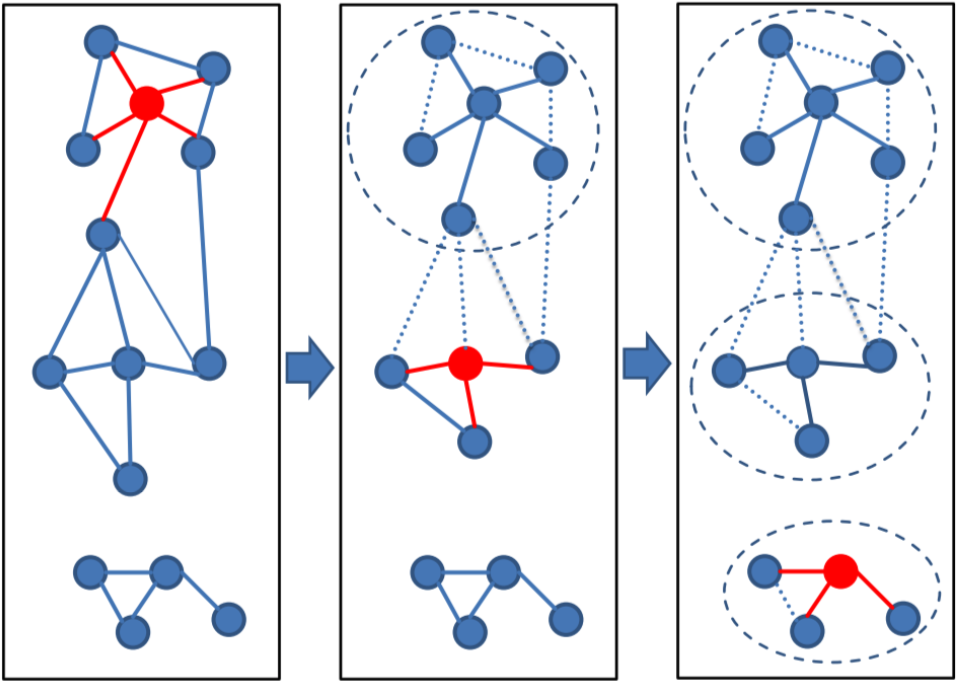
\includegraphics[width=.3\textwidth]{images/cluster-mode-setcover.png}
    \label{fig:set-cover}}
    \hfill
    \subfloat[Connected component]{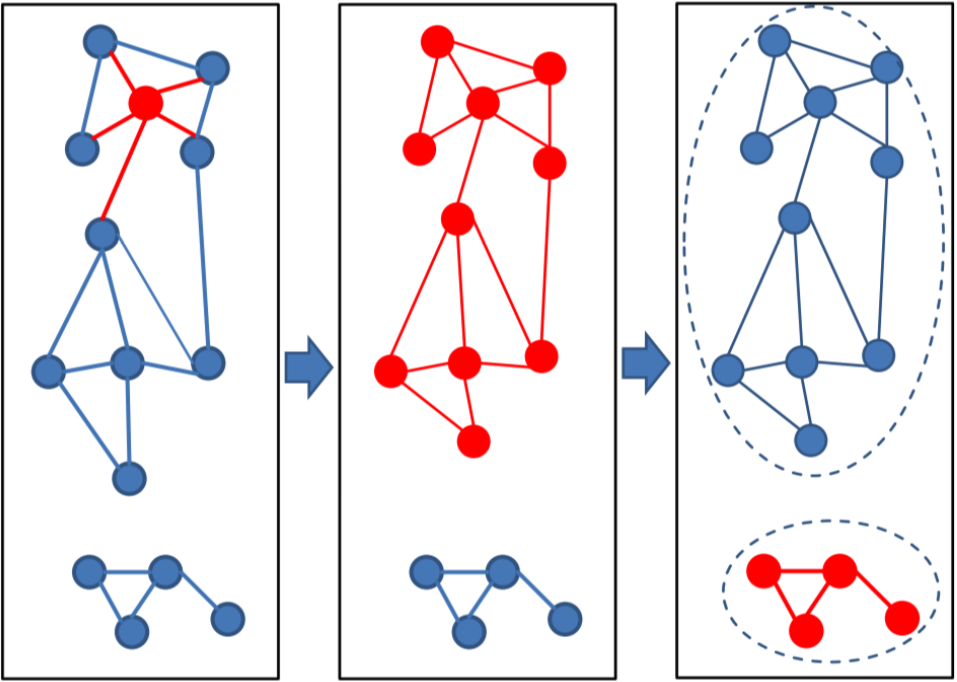
\includegraphics[width=.3\textwidth]{images/cluster-mode-connectedcomp.png}
    \label{fig:connected-componet}}
    \hfill
    \subfloat[CD-hit like]{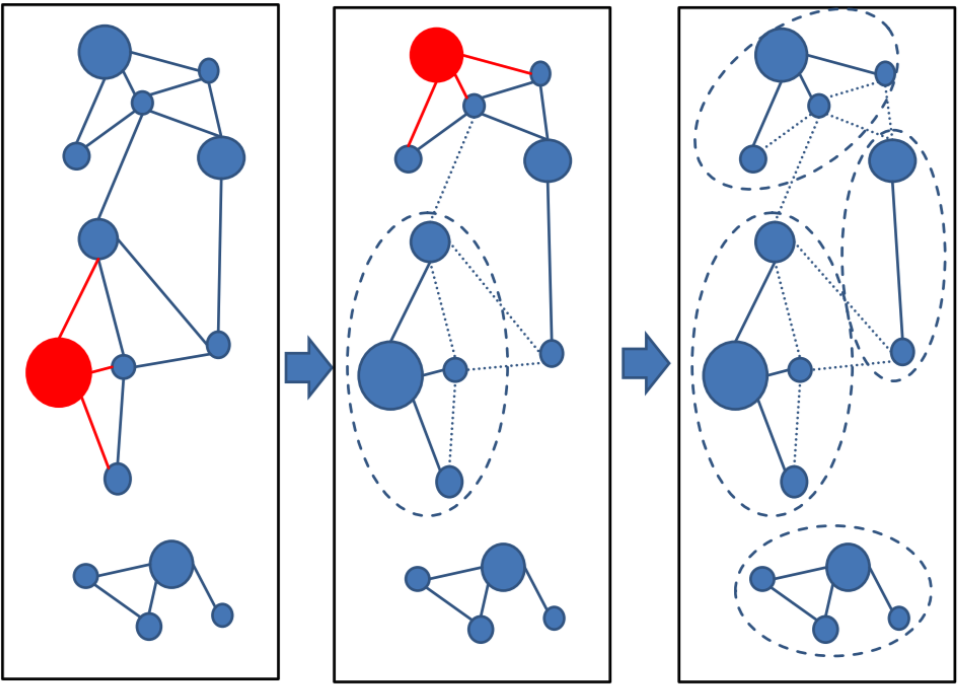
\includegraphics[width=.3\textwidth]{images/cluster-mode-greedyincremental.png}
    \label{fig:cdhit}}
    \caption[Algorithmes de clustering de MMSeqs2]{Algorithme de clustering de MMSeqs2}
    \label{fig:mmclust}
\end{figure}

Depuis 2018, MMSeqs2 intègre une nouvelle méthode appelée Linclust \cite{steinegger_clustering_2018}. Son objectif est de proposer une méthode de clustering des séquences dont le temps évolue linéairement avec le nombre de séquences. Pour ça, les séquences ne seront pas alignées entre elles. Dans un graphe, chaque séquence constitue un n\oe ud et est représentée par des k-mers, qui seront eux partitionnés en groupe de k-mers. La séquence la plus longue du groupe est comparée à toutes les autres séquences du groupe. Si l'alignement dépasse le seuil fixé, alors une arête de similarité est créée entre les séquences. Puis un algorithme de partitionnement est appliqué sur le graphe résultant pour obtenir le partitionnement final. Cette optimisation supplémentaire permet de rapidement partitionner de grands jeux de séquences.

\subsubsection{Modélisation des séquences similaires : matrice de position, profil et chaine de Markov}

Une fois les séquences regroupées par similarité, il est possible de créer un modèle statistique représentant les séquences, sous forme de "séquence" consensus. L'idée générale de ces modèles va être, pour chaque position de la séquence consensus, d'associer pour chaque type de résidus une fréquence ou probabilité d'apparition, basée sur un alignement multiple des séquences.

Les premiers modèles était sous forme de matrice de score à position spécifique (PSSM, position-specific scoring matrices). Les résidus (nucléotide ou acide aminé) en ligne et les positions en colonnes, et chaque valeur représente la fréquence du résidu à cette position pour le groupe de séquences. Les fréquences sont normalisées par la fréquence globale du résidu pour obtenir un score résidu/position indépendant de la longueur et de la composition globale des séquences. Pour terminer, les scores sont convertis en probabilités en appliquant un logarithme. La matrice obtenue reflète pour un score positif une correspondance de résidus similaires parmi les séquences, ou pour un score négatif un résidu non conservé. Ces matrices ont été utilisées dans des outils comme CLUSTAL \cite{higgins_clustal_1988} , MATCH$^{TM}$ \cite{kel_matchtm_2003} pour la recherche de facteur de transcription dans les séquences d'ADN, ou encore dans l'algorithme ESAsearch \cite{beckstette_fast_2006} pour rechercher des séquences dans les PSSMs. Ces outils vont également amener une variante aux PSSMs qui comble un défaut de ces dernières. En effet, le score dépend du nombre et de la divergence des séquences utilisé dans le MSA. Si la matrice est constituée de peu de séquences ou si des séquences proches sont surreprésentées, alors le score sera biaisé. C'est pourquoi un poids est appliqué pour réduire l'impact des séquences proches et augmenter celui des séquences divergentes. 

Pour construire une PSSMs, les MSA doivent être continues (sans \textit{gap}), ce qui est rarement le cas. Une nouvelle forme de PSSM, appelé profile, va alors émerger et prendra en compte les \textit{gap} en appliquant des pénalités. Un profil est donc un PSSM intégrant les possibles indels sous forme de pénalité\footnote{Dans la littérature, les PSSM sont souvent également appelés profile.}. Les profils sont utilisés, notamment dans le contexte des bases de données, pour rechercher des séquences homologues à un groupe de séquence sans aligner chacune des séquences du groupe. PSI-BLAST \cite{altschul_gapped_1997}, développé par les auteurs de BLAST, permet de construire et de rechercher des séquences contre un profil. Pour construire des profils depuis un ensemble de séquences, PSI-BLAST va opérer un cycle dans lequel il va : (\textit{i}) aligner une séquence, en utilisant BLAST, contre toutes les autres séquences, puis garder les meilleurs hits pour construire le profil, (\textit{ii}) de manière itérative, il va aligner ce profil aux séquences restantes pour ajouter des séquences au MSA pour reconstruire un profil, (\textit{iii}) lorsque aucune nouvelle séquence n'est ajoutée au profil alors le cycle reprend avec les séquences restantes. PSI-BLAST est connue pour être hautement sensible, mais également pour être sensible aux séquences mal assignées dans les premières étapes qui vont créer des profils biaisés pour l'ensemble des cycles et des itérations. Pour parer ce problème de "dérapage", il est recommandé de limiter le nombre d'itérations à 3 ou 5.

Une dernière forme de modèle s'appuie sur les chaînes de Markov cachée (HMMs). Une chaîne de Markov décrit la probabilité de transition vers un état en fonction des états précédents. Dans nos modèles, cela correspondrait à calculer la probabilité d'un résidu (état) à une position donnée en fonction des résidus des positions précédentes. Une chaîne de Markov cachée inclut, en plus, l'existence de facteurs non observables sur la probabilité de transition. Dans nos modèles, ces facteurs cachés peuvent être les \textit{gaps} qui ne correspondent à aucun résidu (état) mais influencent la probabilité de transition. On peut alors obtenir une probabilité pour chaque résidu à chaque position. Les modèles HMMs semblent donc tout indiqués pour représenter l'alignement des séquences similaires. Les HMMs, ont l'intérêt de pouvoir différencier les événements d'insertion des événements de délétion par rapport aux profils. Cet avantage les rend plus robustes que les profils. Un outil largement utilisé pour construire des HMMs et rechercher des séquences homologues contre une base de données HMMs est HMMER (\url{http://hmmer.org/}). Un autre outil est HH-suite \cite{steinegger_hh-suite3_2019} qui intègre la possibilité de faire des comparaisons HMM/HMM. Ces outils ont dans leur version récente réussi à s'optimiser pour combler la complexité sous jas cente de l'utilisation de tels modèles. D'autres outils récents, comme ApHMM \cite{firtina_aphmm_2024}, propose des améliorations techniques pour améliorer l'efficacité et la sensibilité des comparaisons aux HMMs, notamment pour ApHMM en s'appuyant sur les nouvelles technologies matérielles et logiciel, et en optimisant les calculs opérés par les algorithmes.

Les modèles HMMs, sont utilisés pour rechercher des séquences homologues dans les bases de données, mais aussi dans d'autres domaines \cite{dimri_hidden_2024} comme la classification et l'annotation des protéines, la prédiction de gènes et de promotteurs\dots